\chapter{Background}\label{chap:background}
\section{Topical location?}
\todo[inline]{Check what better term there is?}
\subsection{Predictive process monitoring:}
Process science revolves around managing and optimizing structured procedures, while the broad area of data science covers data mining, algorithmic analysis and predictive analytics. 
Bridging the gap between the two fields is process mining \cite[p.18]{Aalst16}.
It covers the three steps of model discovery, conformance checking and model enhancement \cite{Aalst16}.

These three steps are focused on offline data.
If one would like to avoid a certain process outcome  or e.g. an SLA violation, a guess at future developments requires resorting to online data analysis.
At this step, techniques from the domain of predictive analytics can be employed\footnote{More detail from Marlon Dumas on how these topics fit together: \url{https://www.youtube.com/watch?v=hMQolsRT0K0}}.

Predictive analytics brings together a variety of statistical techniques like data mining, predictive modelling, and machine learning in order to make predictions about future events throught the use of historical data.
In the domain of business processes, statistical or machine learning models are trained with historical process execution logs and \textit{target} a specific piece of data that should be predicted.
This application is called predictive process monitoring and allows answering questions such as \textit{Given the current state of things, will I still meet my SLA?} or \textit{Given the current case state, how long is this case still going to take?}.
The answers to such questions can give case managers the opportunity to intervene if a case takes an unwanted course or might fail to meet KPI requirements.

\section{Knowledge Discovery in Databases}
\begin{figure}
	\centering
	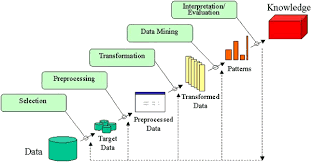
\includegraphics[width=20em]{gfx/kdd_process}
	\caption{The process for \textit{Knowledge Discovery in Databases}}
	\label{fig:kdd_process}
\end{figure}
Predictive analytics is a lot about model training, and the rough outline of necessary steps necessary to train a model is listed here:
\begin{enumerate}
	\item Determine the \textit{target} variable, it is the variable that is supposed to be predicted
	\item Preprocess the dataset. This can mean introducing one-hot encodings, normalized values, but also basic data quality assurance such as null value elimination. Feature engineering can also happen at this step.
	\item Partition the dataset into two parts. One part is set aside for model performance verification, as there the actual target variable value is known. This is commonly referred to as the \textit{test set}, while the remainder is called the \textit{training set}.
	\item Train the model on the training set. Models are trained multiple times with different hyper-parameters to find the optimum configuration with respect to prediction accuracy on the test set. Hyper-parameters are model-specific values such as cutoff-thresholds that have impact on model performance.
\end{enumerate}

\section{Sequence prediction}
\subsection{Sequence-to-Sequence}
\subsection{Word-to-sequence}

\section{Sequence data inputs}
\subsection{Sliding Window}
\subsection{N-gram}
\subsection{Bag-Of-Words}
\subsection{Learned features, word2vec}
Strictly piecewise\\
subsequences

\section{Neural networks}
\subsection{RNN}
\subsection{LSTM memory}
encoding decoding layers with long short-term memory An artificial neural network is an example for a machine learning model. It is made up of neurons, similar to its organic counterpart. The network is organized in three types of layers: a single input layer, one or more hidden layers and a single output layer.
The neurons (being mathematical functions), pass their output on to those in the next layer via weighted connections. The weights on these connections are changed as the network is trained \cite{rosenblatt1958}.
Improving this forward-feeding network with backpropagation, i.e. learning from errors, made applications on pattern-detection successful\footnote{Backpropagation can be attributed to many authors, as Schmidhuber blogs: \url{http://people.idsia.ch/~juergen/who-invented-backpropagation.html}}.
Finally, enhancing the network with a way to remember sequences of events allows application on time-series data. The capacity as well as the durability of this memory are purposely limited as to avoid overfitting.
As such, a long short-term memory inside a neural network functions similarly to our human one: we can remember a certain number of things for a short time, but we do forget some of them.
The LSTM feature also equips the network with a remember and a forget capacity \cite{hochreiter1997}.